\documentclass[12pt,a4paper]{article}

\usepackage{iftex}
\ifPDFTeX
    \usepackage[utf8]{inputenc}
    \usepackage[T5]{fontenc}
    \usepackage[utf8]{vietnam}
\else
    \usepackage{fontspec}
    \IfFontExistsTF{Arial}{
        \setmainfont{Arial}
    }{
        \IfFontExistsTF{TeX Gyre Termes}{
            \setmainfont{TeX Gyre Termes}
        }{
            \setmainfont{Latin Modern Roman}
        }
    }
\fi
\usepackage[a4paper,margin=2.5cm]{geometry}
\usepackage{graphicx}
\usepackage{xcolor}
\usepackage{booktabs}
\usepackage{array}
\usepackage{float}
\usepackage{fancyhdr}
\usepackage[unicode]{hyperref}
\usepackage{titlesec}
\usepackage{amsmath}
\usepackage{caption}

\definecolor{Primary}{HTML}{1E3A8A}
\definecolor{Accent}{HTML}{0F766E}
\definecolor{Soft}{HTML}{EEF2FF}

\hypersetup{
    colorlinks=true,
    linkcolor=Primary,
    urlcolor=Accent,
    citecolor=Primary,
    pdftitle={Báo cáo dự đoán điểm cuối kỳ},
    pdfauthor={Đặng Minh Nhiên}
}

\pagestyle{fancy}
\fancyhf{}
\lhead{Dự đoán điểm cuối kỳ}
\rhead{Đặng Minh Nhiên}
\cfoot{\thepage}
\renewcommand{\headrulewidth}{0.4pt}

\titleformat{\section}{\Large\bfseries\color{Primary}}{\thesection}{0.8em}{}
\titleformat{\subsection}{\large\bfseries\color{Accent}}{\thesubsection}{0.8em}{}
\captionsetup{font=small,labelfont=bf}

\begin{document}

\begin{titlepage}
    \centering
    \vspace*{0.6cm}
    {\Large\bfseries TRƯỜNG ĐẠI HỌC\par}
    \vspace{0.25cm}
    {\large KHOA CÔNG NGHỆ THÔNG TIN\par}
    \vspace{1.2cm}
    \rule{\textwidth}{1.2pt}
    \vspace{0.9cm}

    {\Huge\bfseries\color{Primary} BÁO CÁO BÀI TẬP\par}
    \vspace{0.45cm}
    {\LARGE\bfseries Dự đoán điểm cuối kỳ bằng TensorFlow Computational Graph\par}

    \vspace{0.9cm}
    \rule{0.78\textwidth}{0.8pt}
    \vspace{1.2cm}

    \begin{tabular}{>{\bfseries}p{4.2cm}p{8.5cm}}
        Môn học: & Cấu trúc dữ liệu và giải thuật nâng cao \\
        Giảng viên: & Nguyễn Thanh Sơn \\
        Sinh viên: & Đặng Minh Nhiên \\
        Dataset: & data/TRAIN2.xlsx \\
        GitHub: & \href{https://github.com/MichaelSkyman/Final_score_prediction}{github.com/MichaelSkyman/Final\_score\_prediction} \\
    \end{tabular}

    \vfill
    {\large \today\par}
\end{titlepage}

\tableofcontents
\newpage

\section{Giới thiệu bài toán}
Bài toán yêu cầu xây dựng chương trình dự đoán điểm cuối kỳ của sinh viên dựa trên điểm giữa kỳ của cùng một môn học.
Dataset sử dụng là \texttt{TRAIN2.xlsx}, gồm 515 mẫu dữ liệu với hai thuộc tính:
\texttt{midterm} là điểm giữa kỳ và \texttt{final} là điểm cuối kỳ.

Đây là bài toán hồi quy một biến vì đầu ra cần dự đoán là một giá trị số liên tục trên thang điểm 0 đến 10.
Mục tiêu của chương trình là học một ánh xạ từ điểm giữa kỳ sang điểm cuối kỳ, đồng thời biểu diễn quá trình tính toán dưới dạng computational graph bằng TensorFlow.

\section{Tiền xử lý dữ liệu}
Dữ liệu được đọc bằng \texttt{pandas} từ file Excel. Chương trình giữ lại hai cột \texttt{midterm} và \texttt{final}, chuyển dữ liệu sang dạng số, loại bỏ giá trị thiếu nếu có, sau đó chia dữ liệu thành tập huấn luyện và tập kiểm tra theo tỷ lệ 80/20 với seed cố định để kết quả có thể tái lập.

\begin{table}[H]
    \centering
    \caption{Tóm tắt dataset}
    \begin{tabular}{lr}
        \toprule
        Nội dung & Giá trị \\
        \midrule
        Số mẫu & 515 \\
        Số mẫu huấn luyện & 412 \\
        Số mẫu kiểm tra & 103 \\
        Điểm giữa kỳ nhỏ nhất / lớn nhất & 0.03 / 9.96 \\
        Điểm cuối kỳ nhỏ nhất / lớn nhất & 2.03 / 9.97 \\
        \bottomrule
    \end{tabular}
\end{table}

\section{Phương pháp dự báo}
\subsection{Mô hình hồi quy tuyến tính}
Với một biến đầu vào là điểm giữa kỳ, mô hình hồi quy tuyến tính được chọn vì đơn giản, minh bạch và phù hợp với yêu cầu thuyết minh bằng công thức toán học.
Gọi \(x\) là điểm giữa kỳ, \(y\) là điểm cuối kỳ thực tế và \(\hat{y}\) là điểm cuối kỳ dự báo.
Mô hình có dạng:

\[
    \hat{y} = b_0 + b_1x
\]

Trong triển khai TensorFlow, đầu vào được chuẩn hóa trước khi đưa vào lớp tuyến tính:

\[
    z = \frac{x - \mu}{\sigma}
\]

\[
    \hat{y} = b + wz
\]

Sau khi huấn luyện, công thức trên được quy đổi về thang điểm gốc:

\[
    \hat{y} = 2.001954 + 0.800015x
\]

Điểm dự báo cuối cùng được giới hạn trong miền hợp lệ:

\[
    final\_pred = \min(10, \max(0, \hat{y}))
\]

\subsection{Hàm mất mát và tối ưu}
Hàm mất mát được sử dụng là Mean Squared Error:

\[
    L = \frac{1}{n}\sum_{i=1}^{n}(\hat{y_i} - y_i)^2
\]

TensorFlow tự động tính gradient bằng cơ chế autodiff/backpropagation. Về mặt toán học, các đạo hàm chính của mô hình tuyến tính là:

\[
    \frac{\partial L}{\partial w} = \frac{2}{n}\sum_{i=1}^{n}(\hat{y_i} - y_i)z_i
\]

\[
    \frac{\partial L}{\partial b} = \frac{2}{n}\sum_{i=1}^{n}(\hat{y_i} - y_i)
\]

Batch Gradient Descent cập nhật tham số theo công thức:

\[
    w \leftarrow w - \alpha \frac{\partial L}{\partial w}
\]

\[
    b \leftarrow b - \alpha \frac{\partial L}{\partial b}
\]

\section{Cài đặt TensorFlow Computational Graph}
Graph được xây dựng bằng TensorFlow/Keras với cấu trúc:

\[
    Input(midterm) \rightarrow Normalization \rightarrow Dense(1) \rightarrow \hat{y} \rightarrow MSE
\]

Trong đó:
\begin{itemize}
    \item \texttt{Normalization}: học \(\mu\) và \(\sigma\) từ tập huấn luyện bằng \texttt{adapt()}.
    \item \texttt{Dense(1)}: biểu diễn phép tính tuyến tính \(\hat{y} = b + wz\).
    \item \texttt{MeanSquaredError}: đo sai số dự báo.
    \item \texttt{Batch Gradient Descent}: mỗi epoch tính loss và gradient trên toàn bộ tập huấn luyện, sau đó cập nhật tham số một lần.
\end{itemize}

\begin{figure}[H]
    \centering
    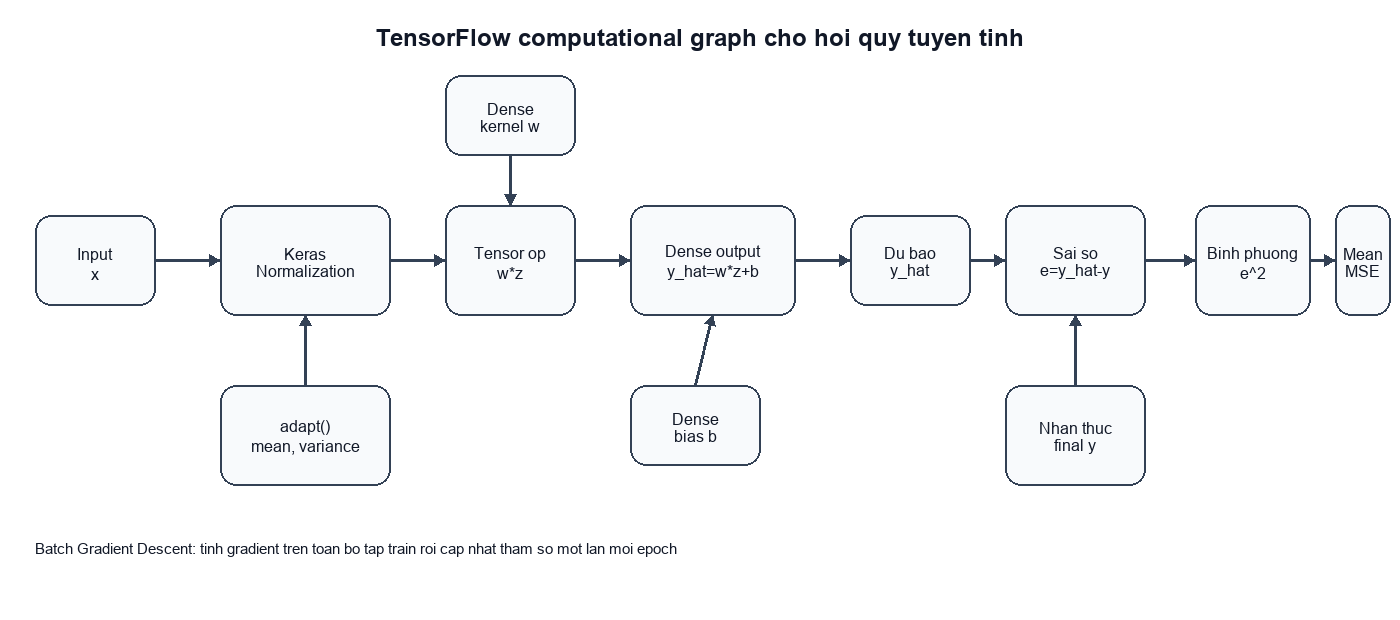
\includegraphics[width=\textwidth]{../outputs/computation_graph.png}
    \caption{Đồ thị tính toán TensorFlow của mô hình hồi quy tuyến tính}
\end{figure}

\section{Kết quả thực nghiệm}
Sau khi huấn luyện bằng TensorFlow graph, mô hình thu được các hệ số:

\begin{table}[H]
    \centering
    \caption{Kết quả mô hình}
    \begin{tabular}{lr}
        \toprule
        Đại lượng & Giá trị \\
        \midrule
        Intercept \(b_0\) & 2.001954 \\
        Slope \(b_1\) & 0.800015 \\
        MAE & 0.002296 \\
        MSE & 0.00000734 \\
        RMSE & 0.002710 \\
        \(R^2\) & 0.999999 \\
        Loss ban đầu & 38.410427 \\
        Loss cuối & 0.00000830 \\
        \bottomrule
    \end{tabular}
\end{table}

Các chỉ số cho thấy điểm giữa kỳ giải thích gần như toàn bộ biến thiên của điểm cuối kỳ trong dataset.
RMSE rất nhỏ, nghĩa là sai số trung bình theo thang điểm gần như không đáng kể trên tập kiểm tra.

\subsection{Nhận xét về mức độ chính xác của mô hình}
Kết quả dự báo có sai số rất nhỏ, gần như không lệch so với dữ liệu thực tế. Đây là một kết quả tốt nhưng cũng cần được nhìn nhận cẩn thận.
Nguyên nhân chính là dataset thể hiện quan hệ tuyến tính rất mạnh giữa điểm giữa kỳ và điểm cuối kỳ, gần với công thức:

\[
    final \approx 2 + 0.8 \times midterm
\]

Do đó mô hình hồi quy tuyến tính học được gần như đúng quy luật sinh dữ liệu:

\[
    final = 2.001954 + 0.800015 \times midterm
\]

Điều này cho thấy mô hình phù hợp với dataset hiện tại. Tuy nhiên, nếu áp dụng cho dữ liệu học tập thực tế hơn, kết quả này có thể hơi lạc quan vì điểm cuối kỳ thường còn phụ thuộc vào nhiều yếu tố khác như bài tập, chuyên cần, mức độ ôn tập, độ khó đề thi và năng lực làm bài cuối kỳ. Vì vậy, khi có thêm dữ liệu độc lập hoặc nhiều thuộc tính hơn, cần kiểm tra lại mô hình để tránh đánh giá quá cao khả năng dự báo.

\begin{figure}[H]
    \centering
    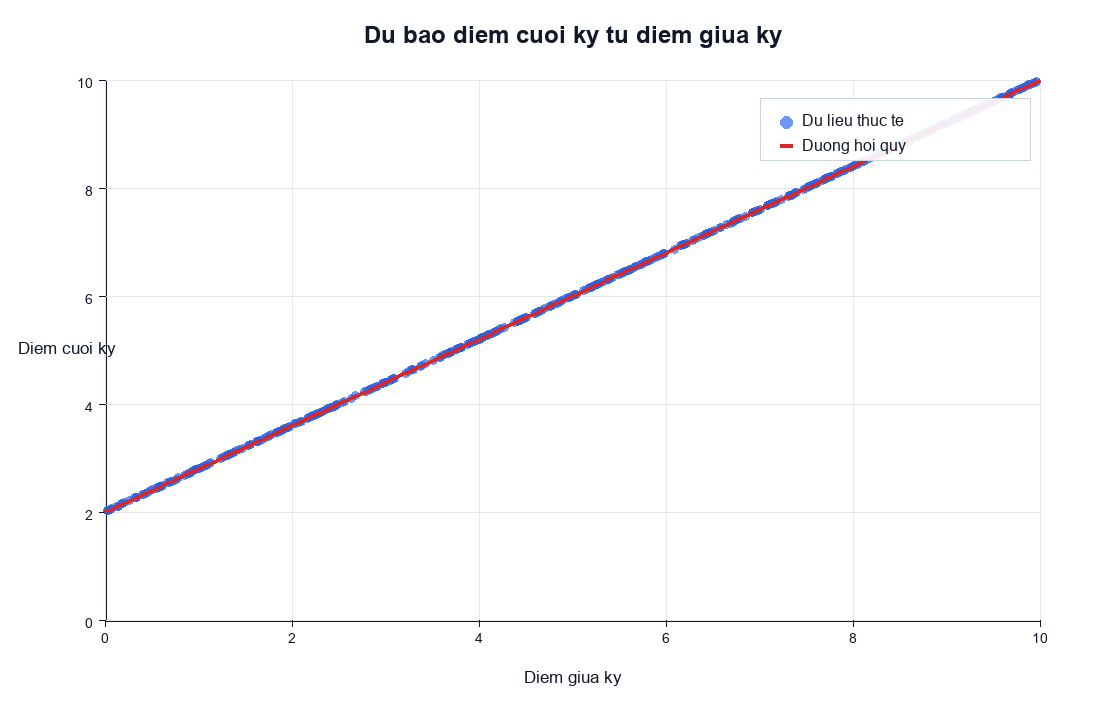
\includegraphics[width=0.92\textwidth]{../outputs/regression_plot.png}
    \caption{Dữ liệu thực tế và đường hồi quy học được}
\end{figure}

\begin{figure}[H]
    \centering
    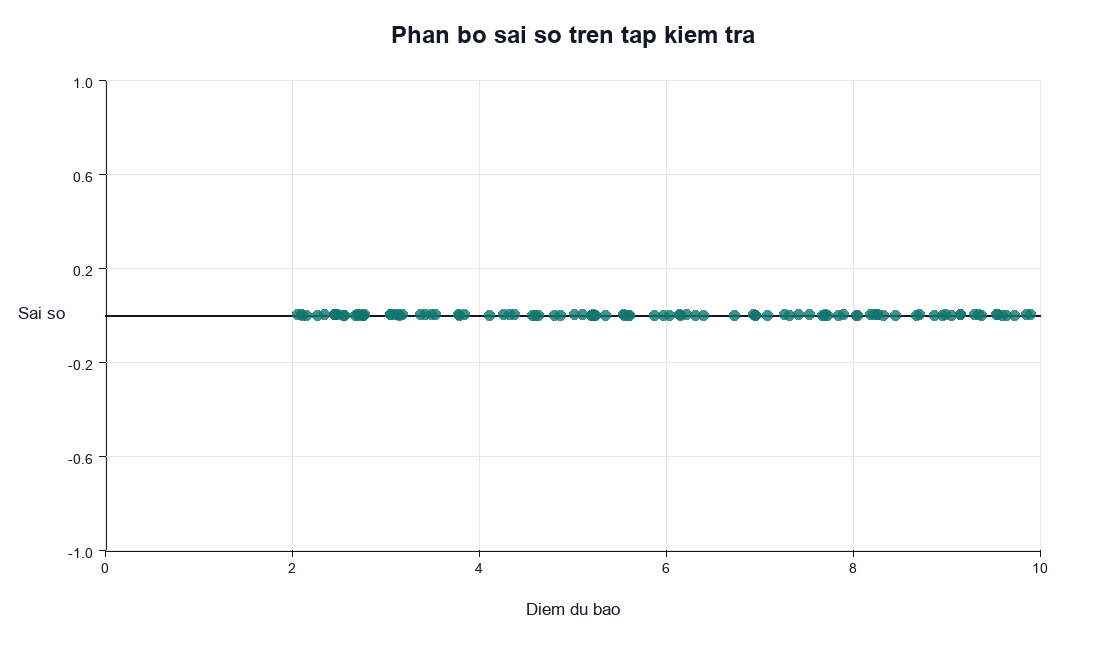
\includegraphics[width=0.92\textwidth]{../outputs/residual_plot.png}
    \caption{Sai số dự báo trên tập kiểm tra}
\end{figure}

\begin{figure}[H]
    \centering
    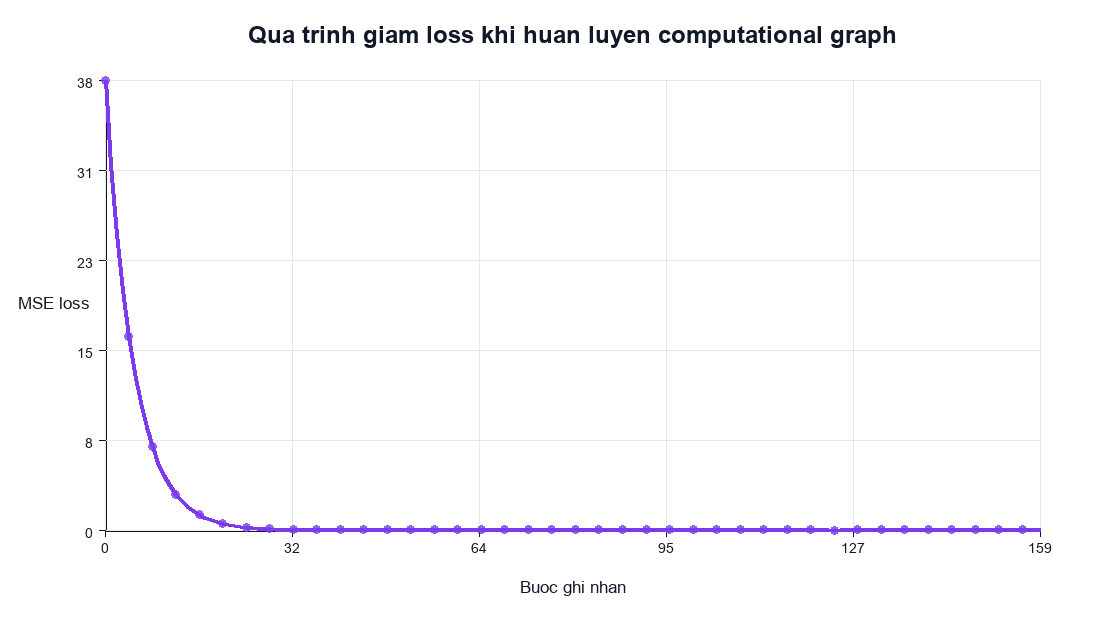
\includegraphics[width=0.92\textwidth]{../outputs/loss_plot.png}
    \caption{Loss giảm trong quá trình huấn luyện TensorFlow graph}
\end{figure}

\section{Cách chạy chương trình}
Mã nguồn được lưu tại:

\[
\href{https://github.com/MichaelSkyman/Final_score_prediction}{https://github.com/MichaelSkyman/Final\_score\_prediction}
\]

Cài đặt môi trường:

\begin{verbatim}
python -m venv .venv
.venv\Scripts\activate
pip install -r requirements.txt
\end{verbatim}

Huấn luyện mô hình và sinh biểu đồ:

\begin{verbatim}
python src/final_score_prediction.py
\end{verbatim}

Dự đoán điểm cuối kỳ cho một điểm giữa kỳ cụ thể:

\begin{verbatim}
python src/final_score_prediction.py --midterm 7.5
\end{verbatim}

\section{Kết luận}
Bài toán dự đoán điểm cuối kỳ từ điểm giữa kỳ được mô hình hóa như một bài toán hồi quy tuyến tính một biến.
Điểm quan trọng của bài là mô hình không chỉ được trình bày dưới dạng công thức, mà còn được cài đặt bằng TensorFlow computational graph.
Graph thể hiện rõ luồng tính toán từ input, chuẩn hóa, lớp tuyến tính, dự báo, hàm mất mát MSE đến quá trình tối ưu bằng Batch Gradient Descent.

Với dataset hiện tại, mô hình đạt sai số rất nhỏ và cho công thức dự báo dễ hiểu:

\[
    final = 2.001954 + 0.800015 \times midterm
\]

\end{document}
